\documentclass[a4paper]{article}

\usepackage[utf8]{inputenc}
\usepackage[T1]{fontenc}
\usepackage{textcomp}
\usepackage{amsmath, amssymb}
\usepackage{float}


% figure support
\usepackage{import}
\usepackage{xifthen}
\pdfminorversion=7
\usepackage{pdfpages}
\usepackage{transparent}
\newcommand{\incfig}[1]{%
	\def\svgwidth{\columnwidth}
	\import{./figures/}{#1.pdf_tex}
}

\pdfsuppresswarningpagegroup=1

\title{NPFL006 Introduction to Formal Linguistics - Homework 5}
\date{\today}
\author{Andrew McIsaac}

\begin{document}
\maketitle
	\begin{figure}[htpb]
		\centering
		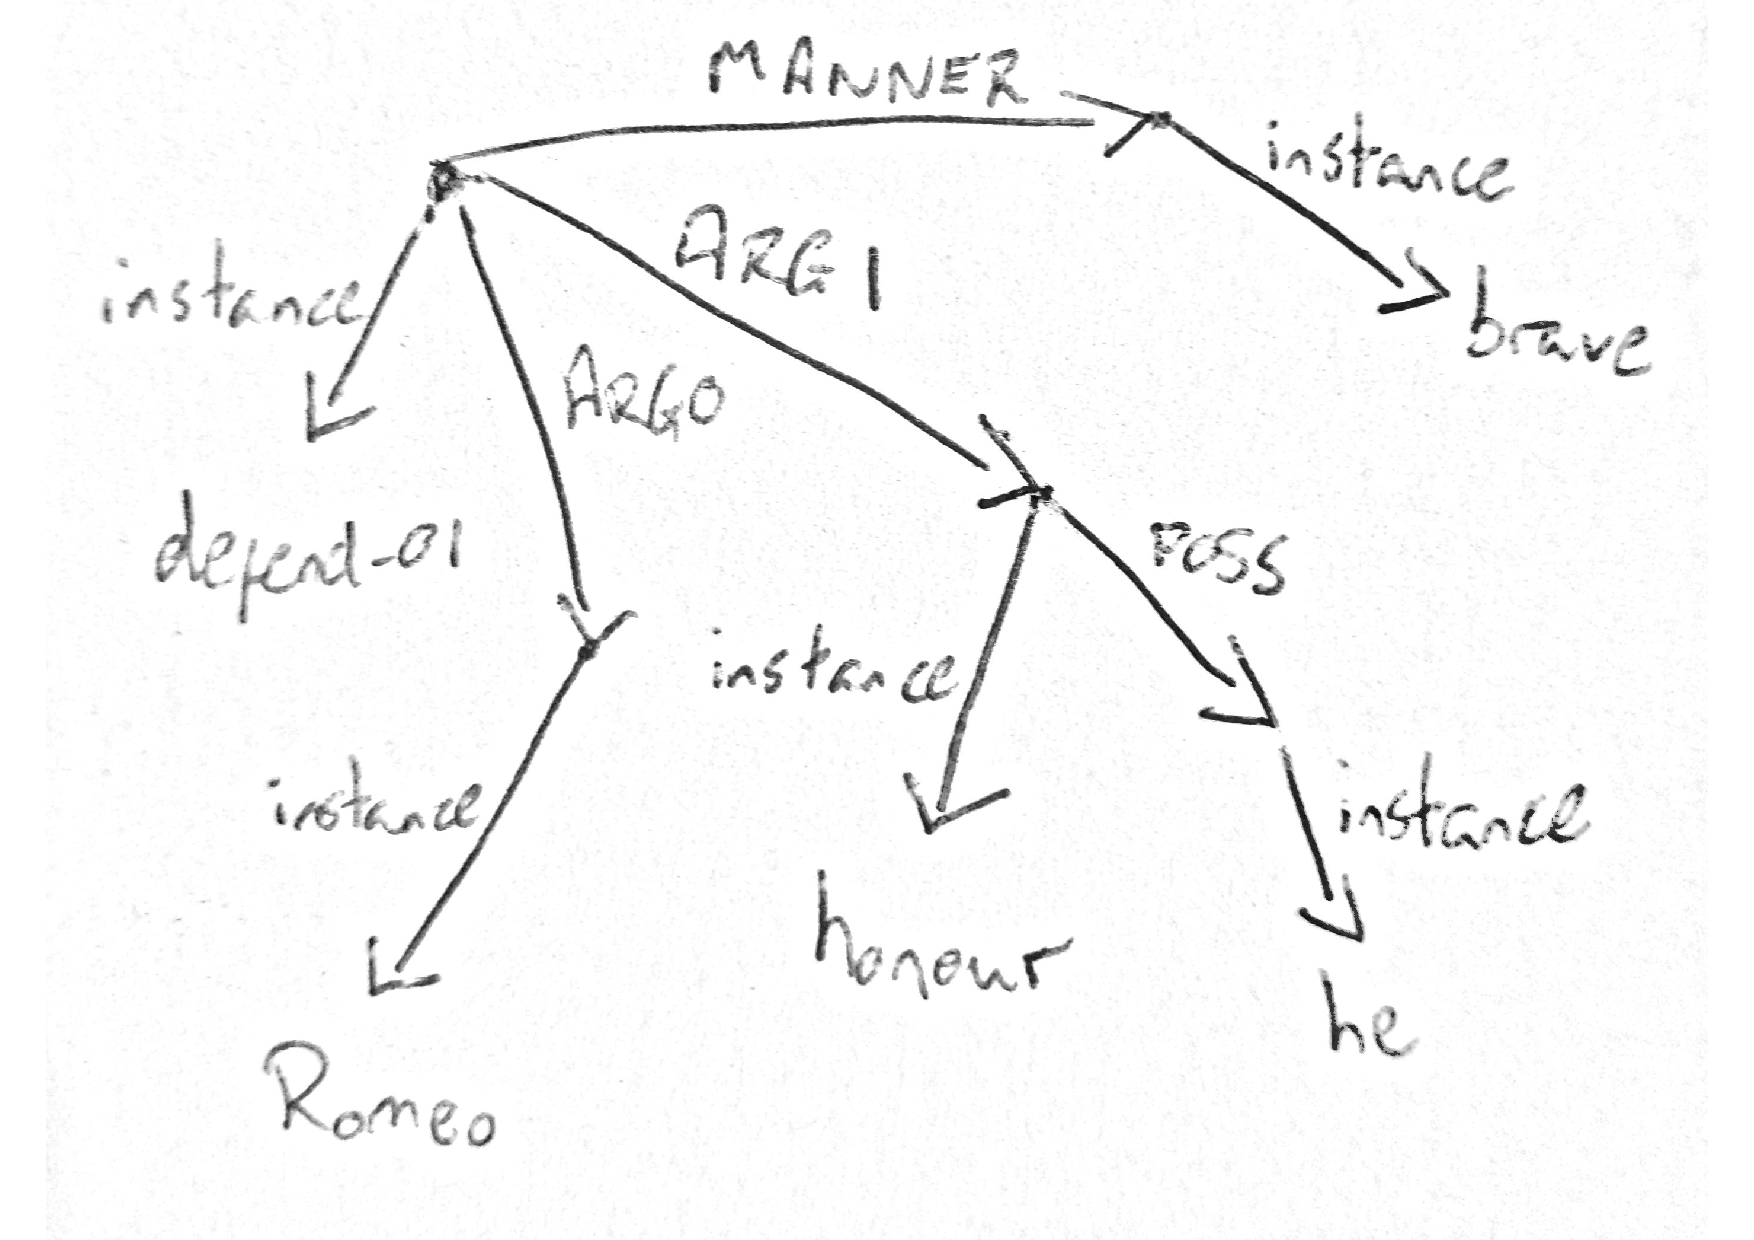
\includegraphics[width=0.8\textwidth]{i_amr}
		\caption{"Romeo defended his honour bravely" in AMR Representation}
		\label{fig:i_amr}
	\end{figure}

	\begin{figure}[htpb]
		\centering
		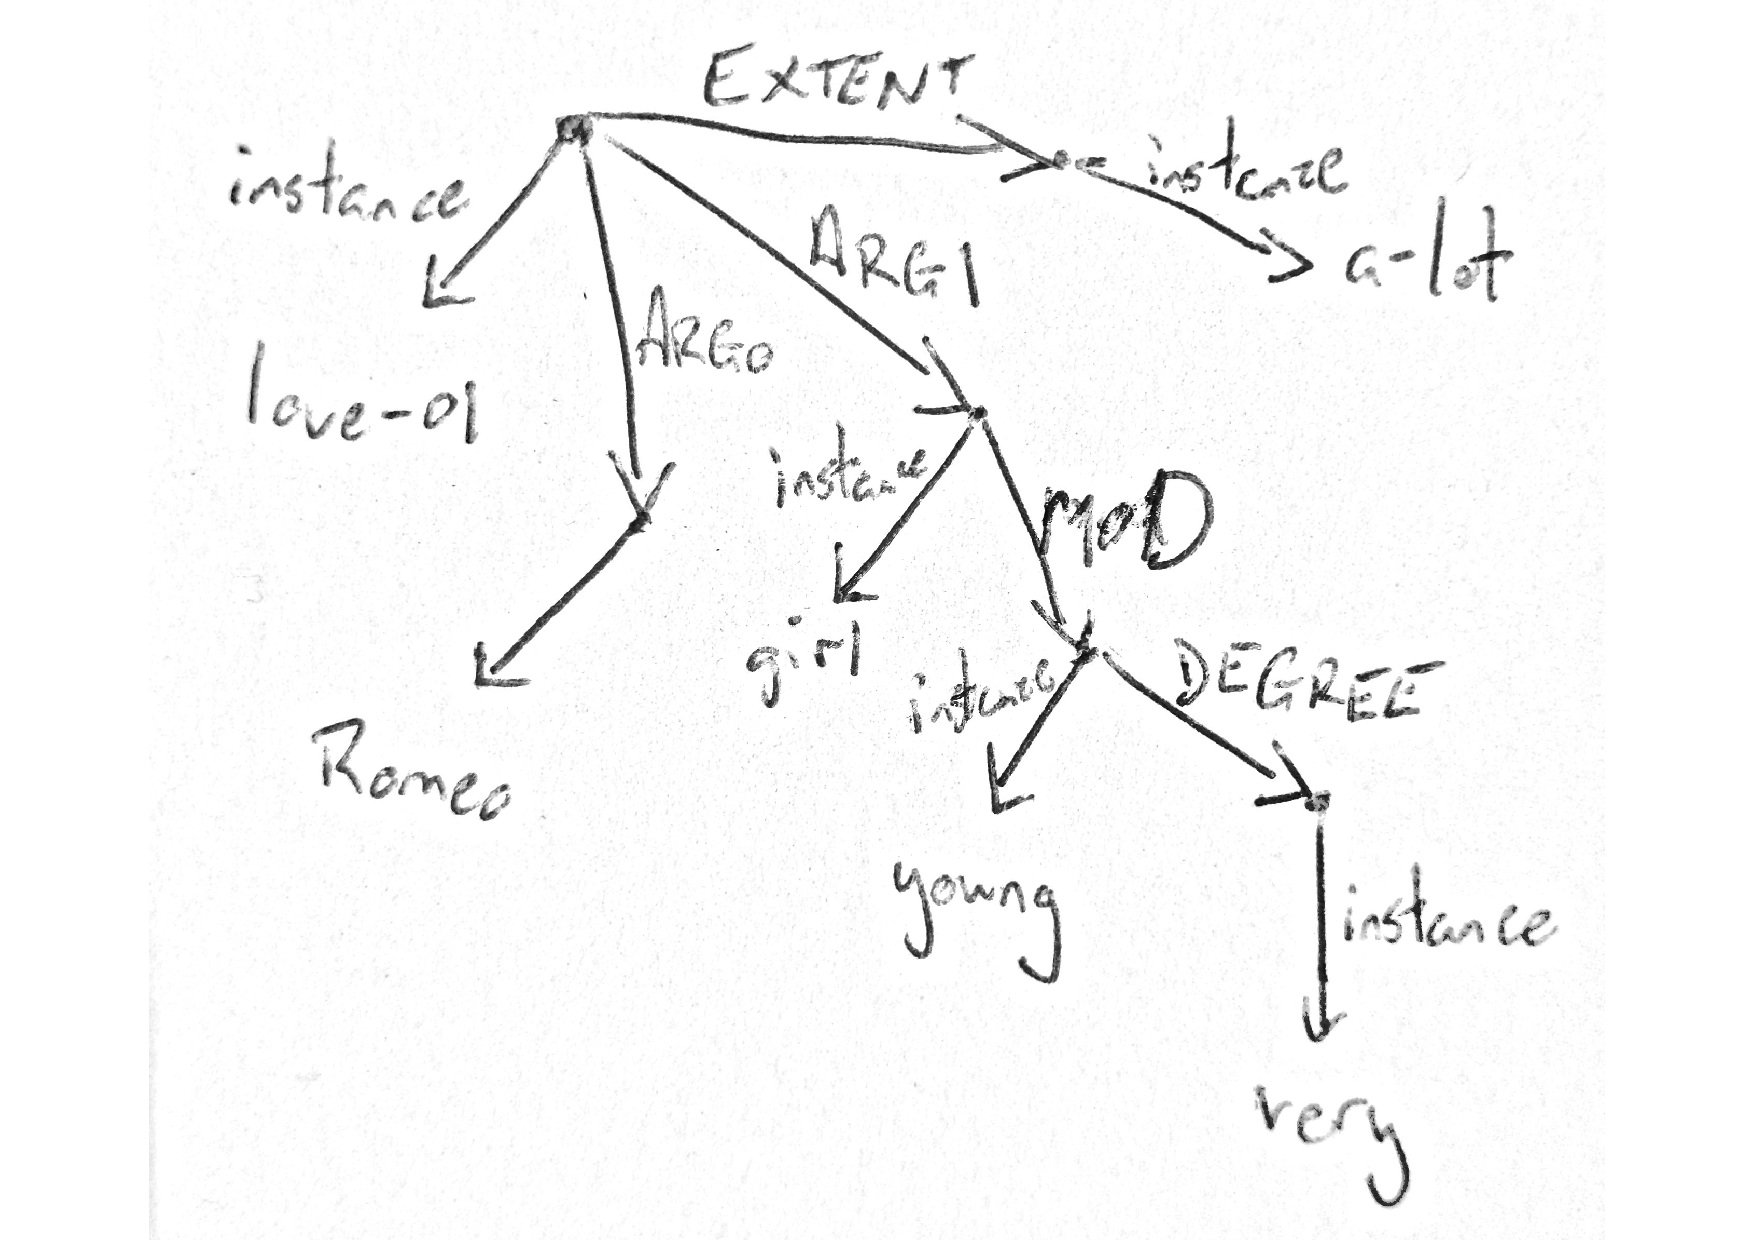
\includegraphics[width=0.8\textwidth]{ii_amr}
		\caption{"The girl Romeo loved so much was very young"
		in AMR Representation}
		\label{fig:ii_amr}
	\end{figure}


	\begin{figure}[htpb]
		\centering
		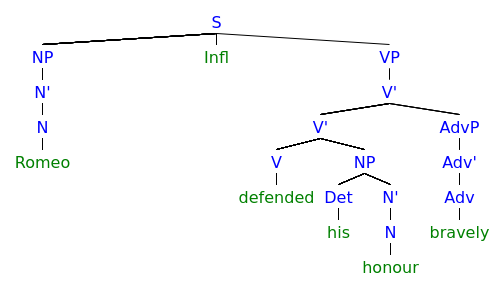
\includegraphics[width=0.8\textwidth]{i_xbar}
		\caption{"Romeo defended his honour bravely" in X-Bar Representation}
		\label{fig:i_xbar}
	\end{figure}

	\begin{figure}[htpb]
		\centering
		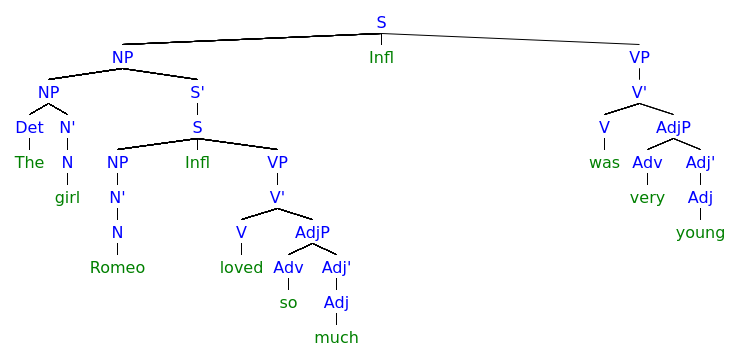
\includegraphics[width=0.8\textwidth]{ii_xbar}
		\caption{"The girl Romeo loved so much was very young"
		in X-Bar Representation}
		\label{fig:ii_xbar}
	\end{figure}
\end{document}
